\chapter{From HOMO--LUMO Levels to Tight-Binding Bands}
\label{ch:homo-lumo-tight-binding}

A finite molecule has discrete molecular orbitals.  A periodic solid has Bloch
bands.  Tight binding connects these descriptions by coupling localized atomic
or molecular orbitals on neighboring sites.  One localized level on each of
$N$ sites produces $N$ one-electron eigenvalues; as $N$ grows, those closely
spaced levels form a band.  The same spectral construction identifies bonding
and antibonding orbitals in a molecule, HOMO and LUMO levels in a finite system,
and valence and conduction bands in a crystal
\cite{kittel2005,yu2010,rudan2015}.

\section{Localized orbitals as a basis}

Let $\ket{j}$ denote a normalized localized orbital centered on site $j$.  The
simplest orthonormal tight-binding basis satisfies
\begin{equation}
  \braket{i|j}=\delta_{ij}.
  \label{eq:tight-binding-orthonormal-basis}
\end{equation}
The on-site energy is
\begin{equation}
  \epsilon_j=\bra{j}\hat H\ket{j},
  \label{eq:tight-binding-onsite-energy}
\end{equation}
and the coupling between distinct sites is
\begin{equation}
  H_{ij}=\bra{i}\hat H\ket{j}.
  \label{eq:tight-binding-hopping-matrix-element}
\end{equation}
A common sign convention writes the nearest-neighbor matrix element as
\begin{equation}
  \bra{j}\hat H\ket{j+1}=-t,
  \qquad t>0.
  \label{eq:tight-binding-hopping-convention}
\end{equation}
The sign convention places the symmetric bonding combination below the
antisymmetric combination.

The tight-binding Hamiltonian is a one-electron Hamiltonian expressed in a
localized basis.  Its eigenvectors are molecular orbitals for a finite cluster
and Bloch orbitals for a periodic crystal.

\section{Two sites: bonding and antibonding orbitals}

For two equivalent sites $A$ and $B$ with on-site energy $\epsilon$, the
Hamiltonian is
\begin{equation}
  H=
  \begin{pmatrix}
    \epsilon & -t\\
    -t & \epsilon
  \end{pmatrix}.
  \label{eq:two-site-tight-binding-matrix}
\end{equation}
The characteristic equation is
\begin{equation}
  \det(H-EI)
  =(\epsilon-E)^2-t^2=0.
  \label{eq:two-site-characteristic-equation}
\end{equation}
The eigenvalues are
\begin{equation}
  E_{\mathrm b}=\epsilon-t,
  \qquad
  E_{\mathrm a}=\epsilon+t.
  \label{eq:two-site-eigenvalues}
\end{equation}
The corresponding normalized eigenvectors are
\begin{align}
  \ket{\mathrm b}
  &=\frac{\ket A+\ket B}{\sqrt2},
  \label{eq:two-site-bonding-state}\\
  \ket{\mathrm a}
  &=\frac{\ket A-\ket B}{\sqrt2}.
  \label{eq:two-site-antibonding-state}
\end{align}
The symmetric state has enhanced amplitude between the sites and is the bonding
orbital.  The antisymmetric state has a node between the sites and is the
antibonding orbital.  Coupling splits one localized energy $\epsilon$ into two
molecular-orbital energies separated by
\begin{equation}
  \Delta E=2t.
  \label{eq:two-site-bonding-antibonding-splitting}
\end{equation}

\begin{figure}[H]
  \centering
  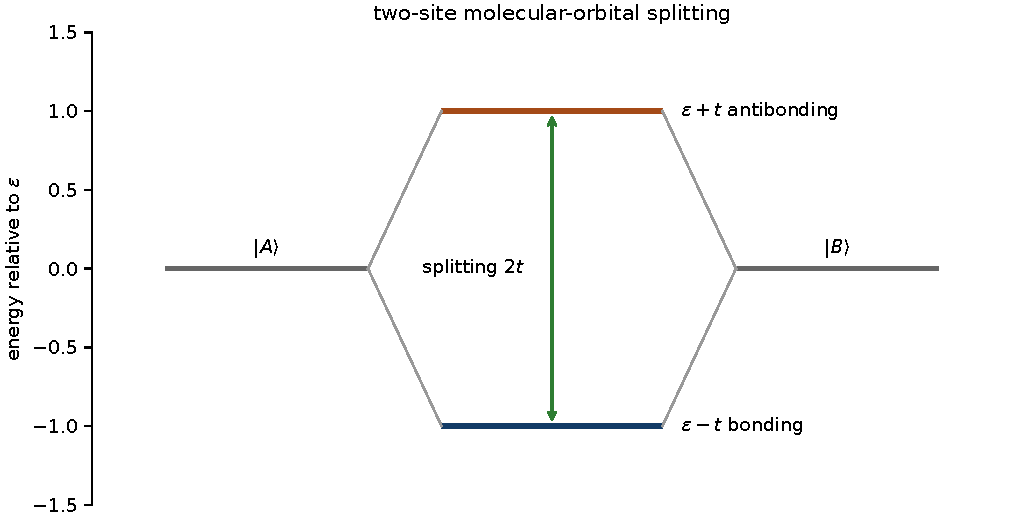
\includegraphics[width=0.84\textwidth]{figures/foundation-two-site-splitting.pdf}
  \caption{Two equivalent localized orbitals at energy $\epsilon$ form a lower
  bonding orbital and an upper antibonding orbital.  The hopping magnitude $t$
  sets the splitting $2t$.\figurenotebookmark}
  \label{fig:foundation-two-site-splitting}
\end{figure}
\figurenotebooktext{figures/02_homo-lumo-tight-binding/fig_02_01.ipynb}

\section{HOMO and LUMO in a finite system}

A finite molecule or cluster has discrete one-electron orbitals
\begin{equation}
  E_1\le E_2\le\cdots\le E_M.
  \label{eq:finite-molecular-orbital-ordering}
\end{equation}
An independent-electron ground-state filling with a prescribed electron number
selects the occupied orbitals.  The highest occupied molecular orbital is the
HOMO, with energy
\begin{equation}
  E_{\mathrm H}=E_{N_{\mathrm{occ}}},
  \label{eq:homo-energy-definition}
\end{equation}
and the lowest unoccupied molecular orbital is the LUMO,
\begin{equation}
  E_{\mathrm L}=E_{N_{\mathrm{occ}}+1}.
  \label{eq:lumo-energy-definition}
\end{equation}
The one-electron HOMO--LUMO gap is
\begin{equation}
  \boxed{
  \Delta_{\mathrm{HL}}=E_{\mathrm L}-E_{\mathrm H}.
  }
  \label{eq:homo-lumo-gap}
\end{equation}
HOMO and LUMO are occupation labels applied to a finite one-electron spectrum.
The spectrum comes from the Hamiltonian; the electron inventory determines
which levels receive those labels.

The one-electron HOMO--LUMO difference is a model energy spacing.  Optical and
charged excitation energies can include relaxation, electron--hole attraction,
and many-body corrections.  Their evaluation requires the corresponding
excitation model.

\section{A finite chain of localized orbitals}

Consider $N$ equivalent sites with open ends.  The nearest-neighbor Hamiltonian
is
\begin{equation}
  \hat H
  =\epsilon\sum_{j=1}^{N}\ket j\bra j
  -t\sum_{j=1}^{N-1}
   \left(
     \ket j\bra{j+1}
    +\ket{j+1}\bra j
   \right).
  \label{eq:open-chain-tight-binding-hamiltonian}
\end{equation}
Write an eigenstate as
\begin{equation}
  \ket{\psi_r}=\sum_{j=1}^{N}c_j^{(r)}\ket j.
  \label{eq:open-chain-eigenstate-expansion}
\end{equation}
The interior coefficients satisfy
\begin{equation}
  -t c_{j-1}^{(r)}+\epsilon c_j^{(r)}-t c_{j+1}^{(r)}
  =E_r c_j^{(r)}.
  \label{eq:open-chain-difference-equation}
\end{equation}
The open boundaries are represented by
\begin{equation}
  c_0^{(r)}=c_{N+1}^{(r)}=0.
  \label{eq:open-chain-coefficient-boundaries}
\end{equation}
The normalized solutions are standing waves on the site index:
\begin{equation}
  c_j^{(r)}
  =\sqrt{\frac{2}{N+1}}
   \sin\left(\frac{r\pi j}{N+1}\right),
  \qquad r=1,\ldots,N,
  \label{eq:open-chain-eigenvectors}
\end{equation}
with energies
\begin{equation}
  \boxed{
  E_r
  =\epsilon-2t
   \cos\left(\frac{r\pi}{N+1}\right).
  }
  \label{eq:open-chain-eigenvalues}
\end{equation}
One localized orbital per site has produced exactly $N$ molecular orbitals.
All energies lie in
\begin{equation}
  \epsilon-2t<E_r<\epsilon+2t.
  \label{eq:open-chain-energy-interval}
\end{equation}
The width approaches
\begin{equation}
  W=4t
  \label{eq:nearest-neighbor-bandwidth}
\end{equation}
as $N$ increases.

\begin{figure}[H]
  \centering
  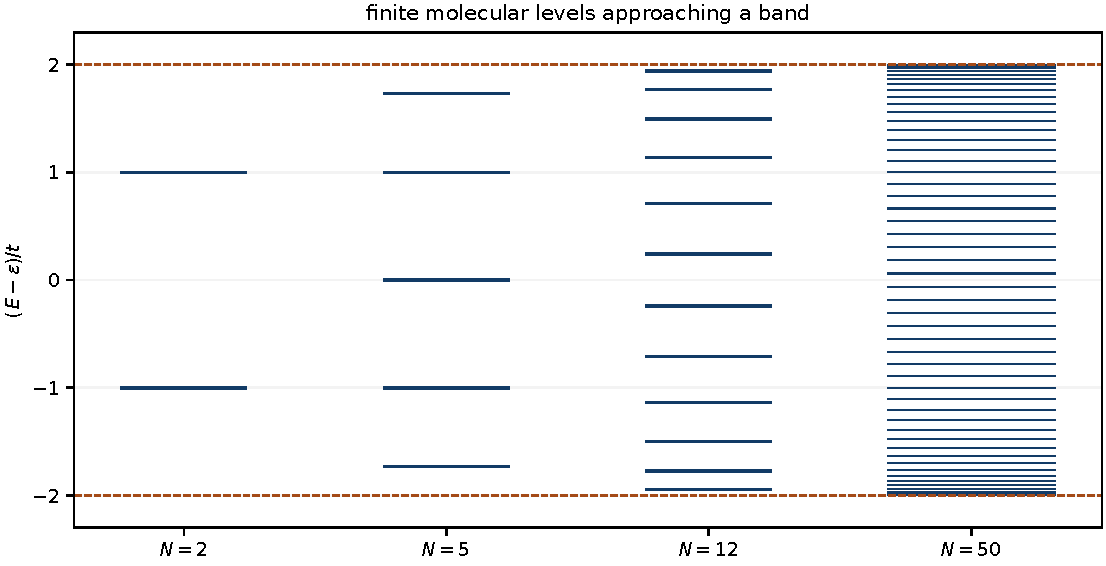
\includegraphics[width=0.90\textwidth]{figures/foundation-levels-to-band.pdf}
  \caption{One localized level on each site produces $N$ molecular-orbital
  energies.  Increasing $N$ fills the finite interval
  $\epsilon-2t<E<\epsilon+2t$ with progressively closer levels.\figurenotebookmark}
  \label{fig:foundation-levels-to-band}
\end{figure}
\figurenotebooktext{figures/02_homo-lumo-tight-binding/fig_02_02.ipynb}

\section{The periodic chain and the Bloch basis}

Join the final site to the first and label sites modulo $N$.  The Hamiltonian is
\begin{equation}
  \hat H
  =\epsilon\sum_{j=0}^{N-1}\ket j\bra j
  -t\sum_{j=0}^{N-1}
   \left(
     \ket j\bra{j+1}
    +\ket{j+1}\bra j
   \right).
  \label{eq:periodic-chain-tight-binding-hamiltonian}
\end{equation}
The normalized Bloch basis is
\begin{equation}
  \boxed{
  \ket k
  =\frac{1}{\sqrt N}
   \sum_{j=0}^{N-1}e^{ikja}\ket j.
  }
  \label{eq:tight-binding-bloch-basis}
\end{equation}
The allowed wave vectors satisfy
\begin{equation}
  k=\frac{2\pi m}{Na}.
  \label{eq:tight-binding-allowed-k}
\end{equation}
Acting with the Hamiltonian gives
\begin{equation}
\begin{aligned}
  \hat H\ket k
  &=\epsilon\ket k
    -t e^{ika}\ket k
    -t e^{-ika}\ket k\\
  &=\left[\epsilon-2t\cos(ka)\right]\ket k.
\end{aligned}
  \label{eq:tight-binding-bloch-diagonalization}
\end{equation}
Therefore
\begin{equation}
  \boxed{
  E(k)=\epsilon-2t\cos(ka).
  }
  \label{eq:nearest-neighbor-tight-binding-band}
\end{equation}
The Bloch transformation is the discrete Fourier transformation from localized
site orbitals to translation eigenstates.  It diagonalizes every
translation-invariant one-orbital nearest-neighbor Hamiltonian.

For finite $N$, equation~\eqref{eq:nearest-neighbor-tight-binding-band} is
sampled at $N$ discrete $k$ values.  In the thermodynamic limit those values
become dense in the first Brillouin zone and the molecular-orbital levels become
a continuous band.

\section{Several orbitals per cell}

Let each primitive cell contain $q$ localized orbitals labeled by $\alpha$.  A
Bloch basis is formed for each orbital:
\begin{equation}
  \ket{\alpha,\bm k}
  =\frac{1}{\sqrt N}
   \sum_{\bm R}
   e^{i\bm k\cdot\bm R}
   \ket{\alpha,\bm R}.
  \label{eq:multiorbital-bloch-basis}
\end{equation}
The Hamiltonian becomes a $q\times q$ matrix at each $\bm k$:
\begin{equation}
  H_{\alpha\beta}(\bm k)
  =\sum_{\bm R}
   e^{i\bm k\cdot\bm R}
   \bra{\alpha,\bm 0}\hat H\ket{\beta,\bm R}.
  \label{eq:multiorbital-bloch-hamiltonian}
\end{equation}
Diagonalization produces $q$ bands,
\begin{equation}
  H(\bm k)u_{n\bm k}
  =E_n(\bm k)u_{n\bm k},
  \qquad n=1,\ldots,q.
  \label{eq:multiorbital-band-eigenproblem}
\end{equation}
One localized orbital per primitive cell produces one band; $q$ localized
orbitals per cell produce $q$ bands before additional spin multiplicity is
counted.

\section{A two-orbital cell and a band gap}

A chain with two orbitals $A$ and $B$ per cell provides the simplest connection
between molecular bonding--antibonding splitting and separated solid-state
bands.  Let $t_1$ couple $A$ and $B$ inside one cell and $t_2$ couple neighboring
cells.  For equal on-site energy $\epsilon$, the Bloch Hamiltonian is
\begin{equation}
  H(k)=
  \begin{pmatrix}
    \epsilon & -(t_1+t_2e^{-ika})\\
    -(t_1+t_2e^{ika}) & \epsilon
  \end{pmatrix}.
  \label{eq:dimerized-chain-bloch-hamiltonian}
\end{equation}
The characteristic equation gives
\begin{equation}
  (E-\epsilon)^2
  =|t_1+t_2e^{ika}|^2
  =t_1^2+t_2^2+2t_1t_2\cos(ka).
  \label{eq:dimerized-chain-characteristic-equation}
\end{equation}
The two bands are
\begin{equation}
  \boxed{
  E_{\pm}(k)
  =\epsilon\pm
   \sqrt{t_1^2+t_2^2+2t_1t_2\cos(ka)}.
  }
  \label{eq:dimerized-chain-bands}
\end{equation}
At the Brillouin-zone boundary $k=\pi/a$,
\begin{equation}
  E_{\pm}\left(\frac{\pi}{a}\right)
  =\epsilon\pm|t_1-t_2|,
  \label{eq:dimerized-zone-boundary-energies}
\end{equation}
so the band gap is
\begin{equation}
  \boxed{
  E_g=2|t_1-t_2|.
  }
  \label{eq:dimerized-tight-binding-gap}
\end{equation}
The finite two-site bonding and antibonding levels have become lower and upper
Bloch bands.  Alternating couplings separate those bands by a gap.

\begin{figure}[H]
  \centering
  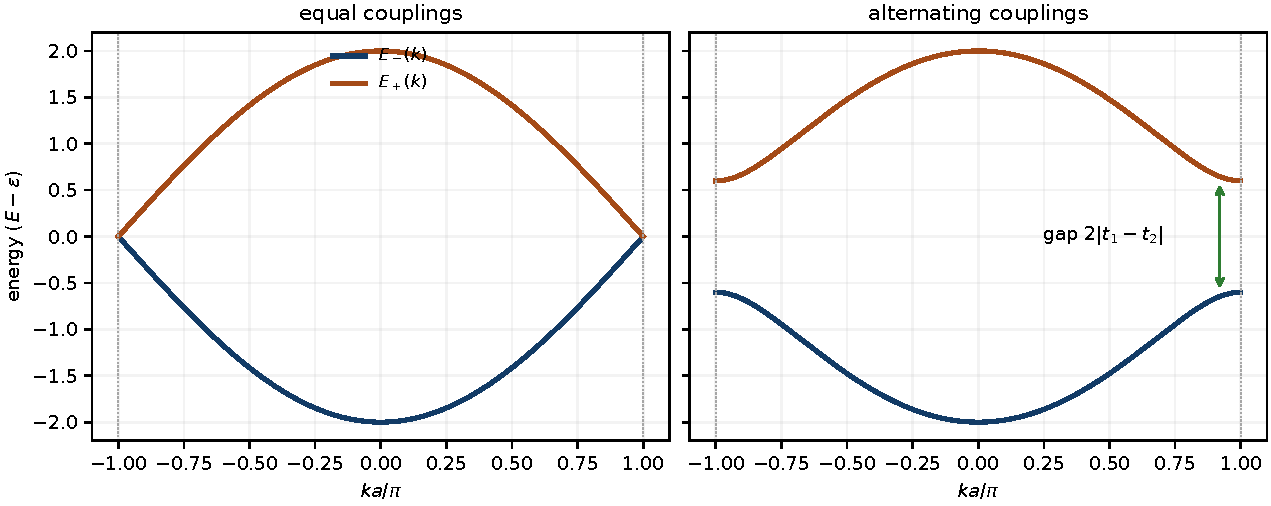
\includegraphics[width=0.88\textwidth]{figures/foundation-dimerized-bands.pdf}
  \caption{Two orbitals per cell produce two Bloch bands.  Equal couplings close
  the gap at the zone boundary; unequal intracell and intercell couplings open
  the gap $2|t_1-t_2|$.\figurenotebookmark}
  \label{fig:foundation-dimerized-bands}
\end{figure}
\figurenotebooktext{figures/02_homo-lumo-tight-binding/fig_02_03.ipynb}

\section{From HOMO and LUMO to valence and conduction bands}

For a finite chain, the electron inventory divides the discrete molecular
orbitals into occupied and empty sets.  Their boundary is the HOMO--LUMO gap.
As the number of cells grows, each family of molecular levels becomes a Bloch
band.  A completely occupied lower band and an empty upper band define a
valence band and conduction band separated by a band gap.

A single spin-degenerate orbital per cell produces one band containing two
one-electron states per cell.  Its electronic character depends on filling.  A
partially filled band has available states at the occupation boundary.  A
completely filled band requires another band to define the lowest empty states
and a possible gap.  The number of orbitals per cell, the hopping matrix, and
the electron inventory jointly determine whether the independent-electron
spectrum is metallic or insulating.

The bulk analogues of HOMO and LUMO are the valence-band maximum and
conduction-band minimum:
\begin{equation}
  E_V=\max_{n\in\mathrm{valence},\bm k}E_n(\bm k),
  \label{eq:valence-band-maximum-from-bands}
\end{equation}
\begin{equation}
  E_C=\min_{n\in\mathrm{conduction},\bm k}E_n(\bm k).
  \label{eq:conduction-band-minimum-from-bands}
\end{equation}
The fundamental independent-particle gap is
\begin{equation}
  \boxed{
  E_g=E_C-E_V.
  }
  \label{eq:fundamental-gap-from-tight-binding-bands}
\end{equation}
The extrema can occur at the same or different wave vectors, producing direct
or indirect gaps.

\section{Model content}

Tight binding preserves the localized-orbital basis, on-site energies, selected
hopping amplitudes, lattice symmetry, and Bloch phase relations.  Additional
orbitals and longer-range hopping extend the spectral range and shape of the
bands.  A nonorthogonal localized basis leads to the generalized eigenproblem
\begin{equation}
  H(\bm k)c_{n\bm k}
  =E_n(\bm k)S(\bm k)c_{n\bm k},
  \label{eq:nonorthogonal-tight-binding-eigenproblem}
\end{equation}
where $S(\bm k)$ is the overlap matrix.  Spin--orbit coupling, magnetism, and
interaction corrections enlarge the Hamiltonian according to the physical
system.

The tight-binding parameters define a reduced one-electron model.  Their
connection to measured or higher-level calculated bands requires an explicit
parameter source and a stated fitting range.

\section{Chapter summary}

Coupling two localized orbitals produces bonding and antibonding molecular
orbitals.  Coupling $N$ sites produces $N$ molecular levels within a finite
energy interval.  Periodic translation diagonalizes the Hamiltonian in a Bloch
basis and converts those levels into the band
$E(k)=\epsilon-2t\cos(ka)$.  Several orbitals per cell produce several bands.
A two-orbital cell shows explicitly how molecular bonding--antibonding splitting
becomes a valence--conduction band separation.  HOMO and LUMO label the occupied
boundary of a finite spectrum; valence- and conduction-band edges provide the
bulk counterpart.  The next chapter uses the spectral representation of these
Bloch bands to derive their density of states.
